\section{xv6调度机制分析}
本章对xv6操作系统中的进程调度机制进行分析。首先介绍xv6进程管理结构及管理结构，然后分析其默认的时间片轮转调度算法及其特点，最后从决策的角度对人物调度进行形式化建模，为后续基于强化学习的调度策略设计提供理论基础。
\subsection{xv6进程管理机制}
\subsubsection{进程模型}
在 xv6 操作系统中，进程（process）是系统资源管理与任务调度的基本单位。xv6 采用简化的进程模型，不区分进程与线程，因此系统中的每个执行实体都以进程的形式存在，并作为调度器进行 CPU 分配的基本对象。

xv6 通过一张全局进程表\texttt{proc[]} 来管理系统中的所有进程。该表本质上是一个固定大小的数组，每个元素对应一个进程控制块（Process Control Block, PCB）。操作系统通过维护该表中的状态信息，实现进程的创建、调度、阻塞与回收等生命周期管理。

在资源管理层面，进程是系统资源的主要持有者。一个进程通常包含以下几类资源：
\begin{itemize}
    \item 地址空间（page table）：描述进程的虚拟内存映射
    \item 寄存器上下文（register context）：保存 CPU 执行状态
    \item 内核栈（kernel stack）：用于系统调用与内核执行
    \item 打开文件表（file descriptors）：管理进程持有的文件资源
\end{itemize}
从操作系统运行状态的角度来看，进程可以被视为一个有限状态机。在其生命周期中，进程会在不同状态之间转换，以配合系统调度与资源管理。xv6 定义了以下几种进程状态：
\begin{itemize}
    \item UNUSED：进程表项未被使用
    \item USED：进程结构已分配但尚未运行
    \item RUNNABLE：进程可运行，等待 CPU 调度
    \item RUNNING：进程正在 CPU 上执行
    \item SLEEPING：进程因等待某事件而阻塞
    \item ZOMBIE：进程已退出但尚未被父进程回收
\end{itemize}
这些状态的转换由调度器、系统调用以及中断机制共同驱动。
\todo[inline]{这里需要一个xv6状态转换图}

在进程组织方式上，xv6 采用 父子进程（parent-child）结构 来管理进程关系。当一个进程调用 \texttt{fork()} 创建新进程时，新进程成为其子进程，并继承部分资源信息。父进程可以通过 \texttt{wait()} 系统调用等待子进程结束并回收其资源，这一机制与 Linux 等现代操作系统的基本进程模型类似。

在实现层面，xv6 使用 \texttt{struct proc} 结构体来描述每个进程的运行状态及其相关信息。该结构体包含：
\begin{itemize}
    \item 进程标识符 pid
    \item 进程状态 state
    \item 内核栈指针
    \item 页表 pagetable
    \item 进程上下文 context
    \item 打开文件表
    \item 父进程指针等信息
\end{itemize}

其中，\texttt{context} 结构用于保存进程在 内核态执行时的寄存器上下文。当调度器发生进程切换时，系统通过 \texttt{swtch()} 函数保存当前进程的寄存器状态，并恢复目标进程的上下文，从而实现不同进程之间的执行切换。

通过上述机制，xv6 实现了一个简洁而完整的进程管理与调度框架，为后续调度算法的实现与扩展提供了基础。
\subsubsection{调度循环}
xv6中进程的调度主要通过 \texttt{scheduler} 进行完成，\texttt{scheduler} 与CPU一一对应，每个CPU再启动后都会进入调度循环，该循环不断扫描系统中的进程表，并选择状态为 \texttt{RUNNABLE} 进程进行执行。
调度器首先遍历系统中的进程数组 \texttt{proc[]}，当发现进程状态为 \texttt{RUNNABLE} 时，将其状态修改为 \texttt{RUNNING} ，并通过上下文切换机制将 CPU 的执行权交给该进程。当进程主动让出 CPU 或发生中断时，控制权重新返回调度器，从而继续进行下一轮调度。
\todo[inline]{调度循环示意图}

\subsubsection{上下文切换机制}
在进程调度过程中，需要在不同进程之间切换CPU的执行上下文，具体来说是进程结构体中的 \texttt{context} 数据结构，其主要包括一些用户寄存器和状态寄存器。xv6通过 \texttt{swtch()} 函数实现上下文切换，该函数通过保存当前进程的寄存器状态，并恢复目标进程的寄存器状态，从而实现执行流在不同进程之间的切换。
在调度过程中，CPU 的上下文保存在 \texttt{struct cpu} 结构中，而进程上下文保存在 \texttt{struct proc} 的 \texttt{context} 成员中。当调度器选择新的进程执行时，系统调用 \texttt{swtch()} 保存当前 CPU 上下文，并恢复目标进程的上下文，从而完成调度切换。
\begin{figure}[htbp]
\centering
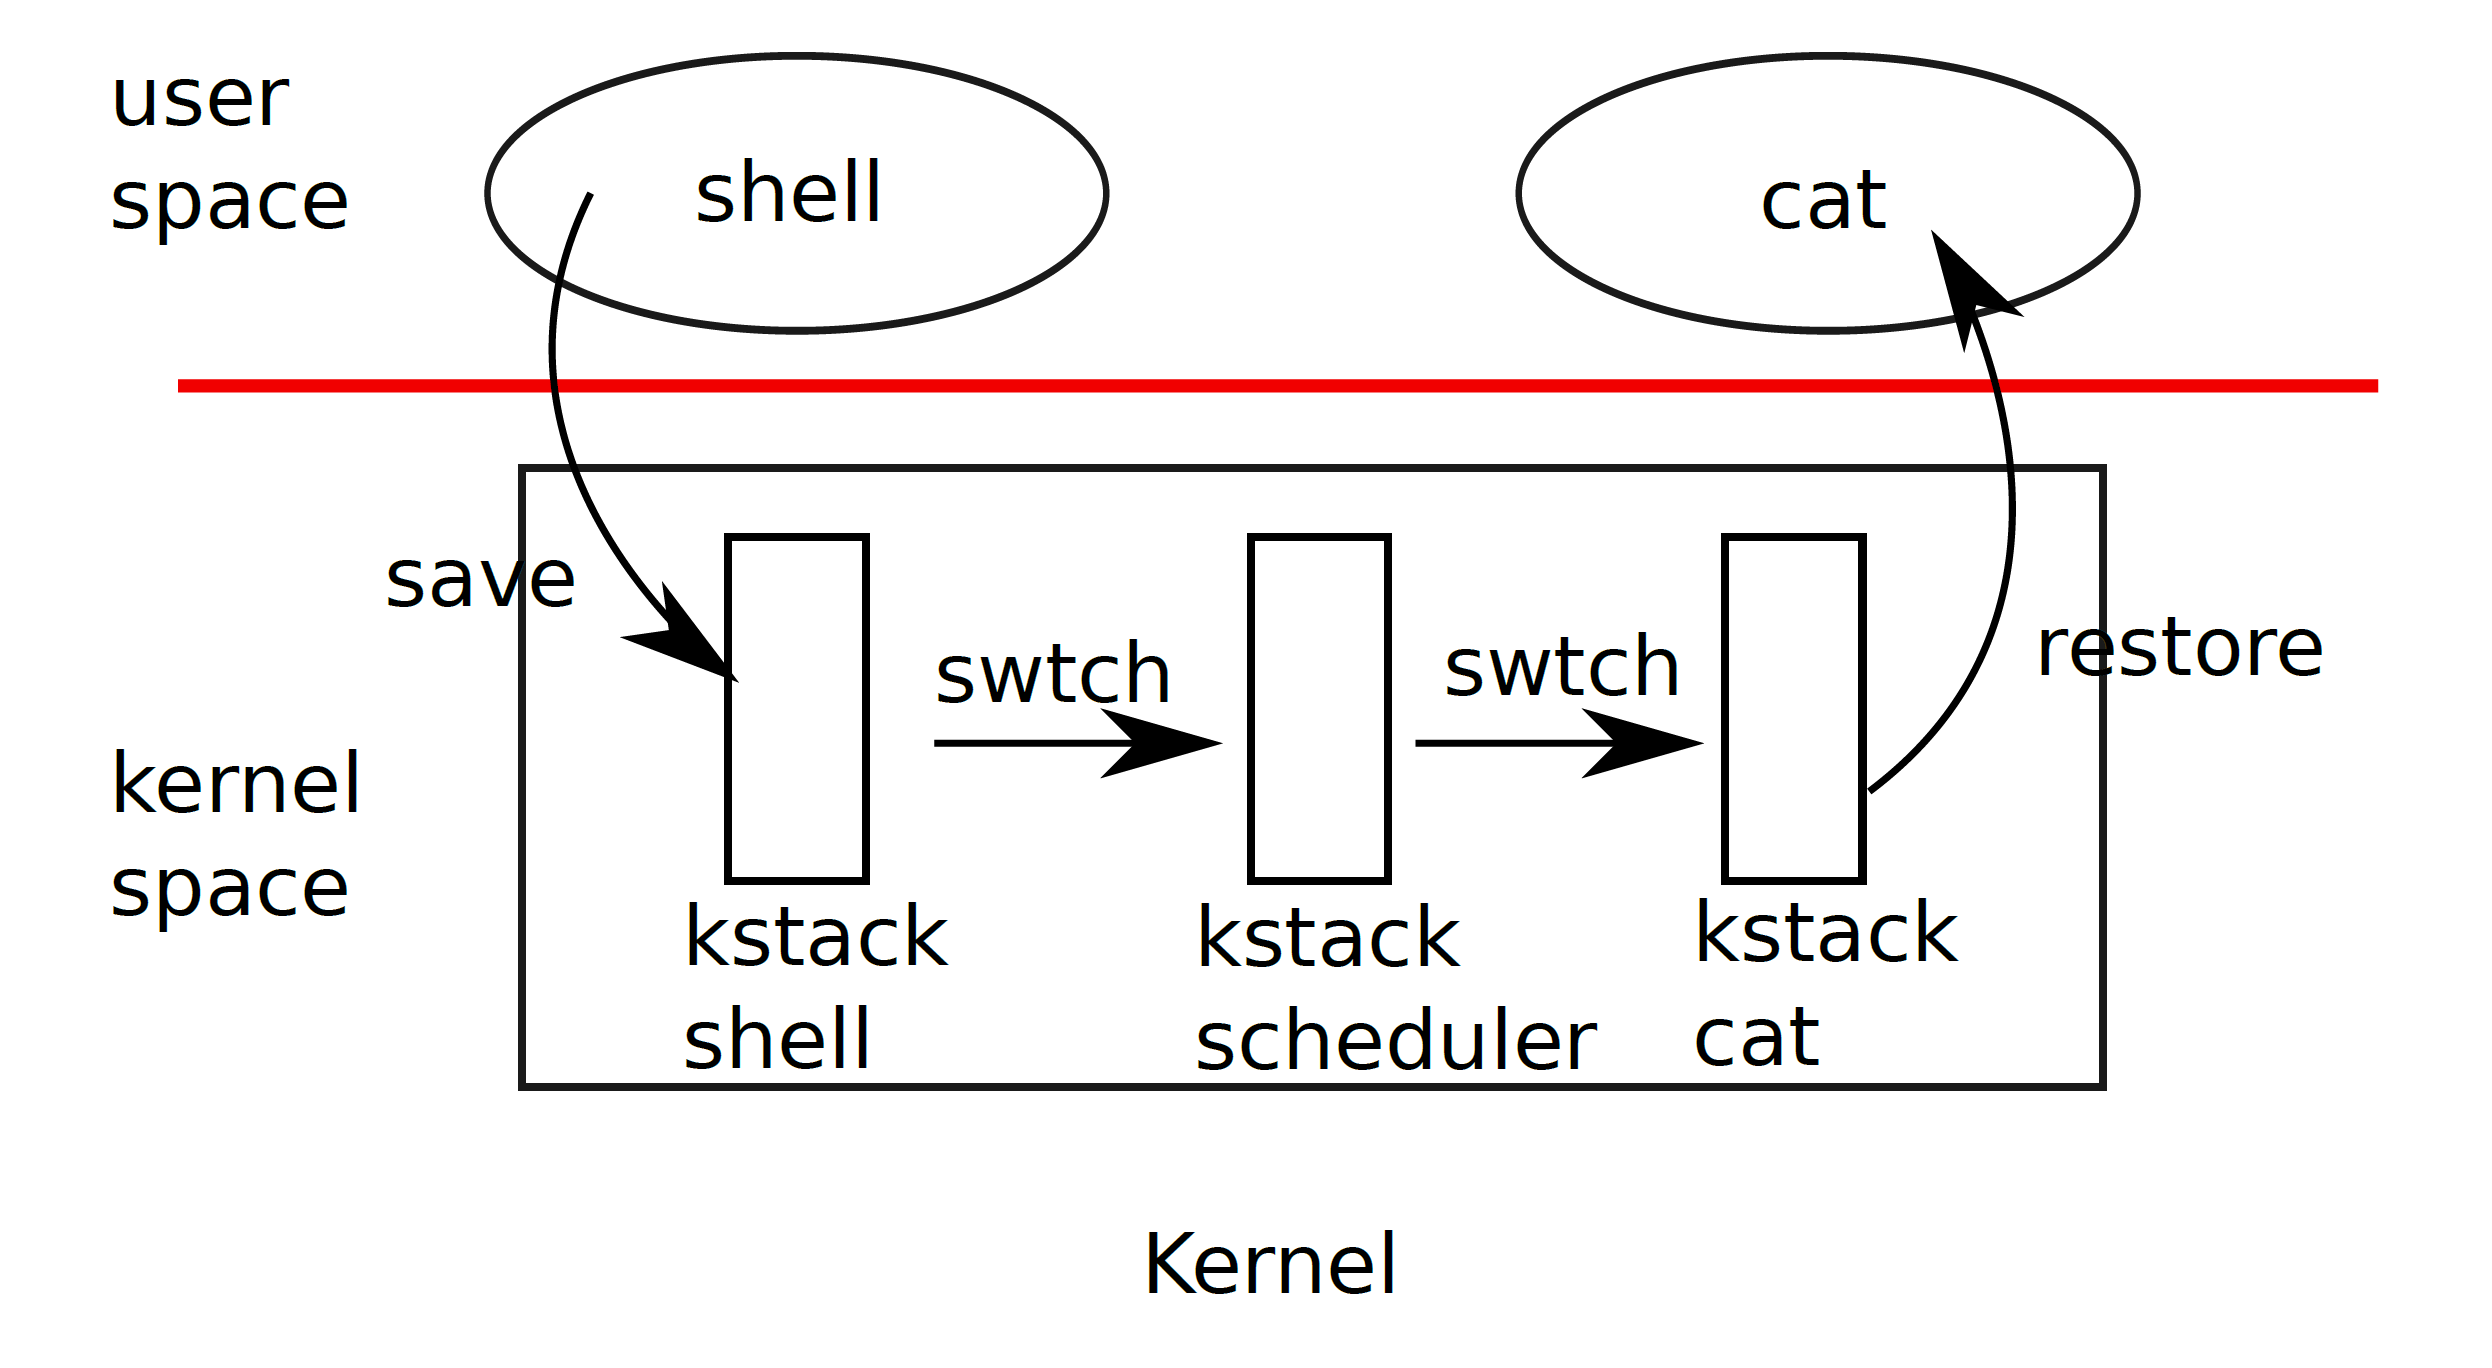
\includegraphics[width=0.7\textwidth]{figures/figure212_1.png}
\caption{xv6 上下文切换机制}
\label{fig:swtch}
\end{figure}

\subsubsection{时钟中断与调度触发}
xv6 的进程之间的切换主要有两种，一种是进程调用 \texttt{sleep} 进如 \texttt{SLEEPING} 或 \texttt{ZOMBIE} 状态，并让出当前的执行机会。另一种依赖于硬件（CPU）所提供的定时器定期产生中断。硬件定时器产生中断时，CPU 会进入内核态并执行中断处理程序。在处理中断的过程中，如果当前进程正在运行，系统会调用 \texttt{yield()} 函数使进程主动让出 CPU，从而触发一次调度。通过这种机制，系统能够实现基于时间片的进程调度，保证多个进程能够共享 CPU 资源。
\todo[inline]{解释图}

\subsection{默认算法分析}
\subsubsection{Round Robin原理}
xv6通过CPU定时器的定时触发功能，默认采用时间片轮转（Round Robin）的调度算法，定时器触发一次是一个时间轮。该算法按照固定顺序遍历进程队列，当发现可运行进程时，将其分配 CPU 执行一个时间片。当时间片结束或进程主动让出 CPU 时，调度器重新选择下一个可运行进程执行。
\subsubsection{算法优缺点}
Round Robin 调度算法具有实现简单、公平性较好的特点，能够保证每个进程在有限时间内获得 CPU 资源，因此被广泛应用于教学操作系统和早期多任务系统中。
尽管时间片轮转调度具有较好的公平性，但该算法采用固定策略进行任务调度，不考虑任务执行特征、系统负载变化以及历史调度信息。因此在复杂计算环境下，其调度效率可能难以达到最优。
\subsubsection{静态策略局限性}
在动态计算环境中，任务执行时间、系统负载以及资源利用率往往具有较大的不确定性。传统的静态调度算法通常依赖于预先设定的规则，难以根据系统运行状态进行动态调整。
因此，需要一种能够根据系统状态进行自适应决策的调度方法，以提高系统整体性能。

\subsection{调度问题的结构建模}
在传统操作系统中，调度策略通常通过固定规则实现，例如时间片轮转（Round-Robin）或优先级调度。这类方法虽然实现简单，但难以根据系统运行状态进行自适应调整。随着强化学习技术的发展，越来越多研究尝试将调度问题建模为序列决策问题，并通过学习算法优化调度策略。

在强化学习框架下，调度问题可以抽象为一个\textbf{马尔可夫决策过程（Markov Decision Process, MDP）}。系统在每一次调度时刻根据当前系统状态选择一个动作（即选择运行的进程），并根据调度结果获得奖励，通过不断交互逐步学习最优策略。

MDP通常由四个元素组成：
$$(S, A, P, R)$$
其中：
\begin{itemize}
    \item S：状态空间（State）
    \item A：动作空间（Action）
    \item P：状态转移概率（Transition）
    \item R：奖励函数（Reward）
\end{itemize}
在操作系统调度问题中，可以对上述元素进行具体定义。
\subsubsection{状态空间}
状态空间用于描述当前系统的运行情况。在任务调度场景中，系统状态可以由多个指标共同构成，例如当前可运行进程数量、各进程的等待时间、运行时间以及历史调度信息等。

在本文的设计中，为了兼顾系统信息表达能力与实现复杂度，状态主要由以下指标构成：
\begin{itemize}
    \item $n$：当前 \textbf{RUNNABLE 进程数量}
    \item $w$： 进程的 \textbf{等待时间（wait time）}
    \item $r$：进程的 \textbf{累计运行时间（run time）}
    \item $c$：进程的 \textbf{调度次数（schedule count）}
\end{itemize}
这些信息可以从 xv6 的 struct proc 结构体中统计得到，并能够反映进程在系统中的运行状态。通过将这些指标组合，可以构建当前调度时刻的系统状态表示。
形式化表示为：
$$s=(n,w,r,c) \in S$$
其中$s$代表系统当前状态。
\subsubsection{动作空间}
在操作系统调度问题中，调度器在每一次调度时刻需要决定选择哪个进程运行。因此动作空间可以定义为：
$$A = 选择某个RUNNABLE进程$$
当系统存在$N$个可运行进程时，动作空间大小为：
$$|A| = N$$
调度器通过选择不同的动作，可以将 CPU 分配给不同进程，从而影响系统运行性能。
\subsubsection{奖励函数}
奖励函数用于评价调度行为对系统性能的影响，是强化学习模型设计中的关键部分。合理的奖励设计可以引导算法学习到更优的调度策略。

在操作系统调度问题中，通常关注以下性能指标：
\begin{itemize}
    \item \textbf{响应时间（Response Time）}
    \item \textbf{等待时间（Waiting Time）}
    \item \textbf{系统吞吐量（Throughput）}
\end{itemize}
为了鼓励调度策略减少进程等待时间并提高系统整体效率，可以设计奖励函数，使得等待时间较短或调度效率较高时获得更高奖励。
例如，可以定义奖励为：
$$r = - waiting\_time$$
或根据多个指标进行组合：
$$r = -\alpha \times waiting\_time + \beta \times throughput$$
其中$\alpha$和$\beta$为权重参数。
通过这种方式，调度器能够在不断交互中学习到能够减少等待时间并提高系统效率的策略。

\subsubsection{调度问题的MDP建模}
在上述定义下，操作系统调度问题可以建模为一个马尔可夫决策过程。

在每一次调度时刻：
\begin{enumerate}
    \item 系统处于某个状态$s$
    \item 调度器根据策略$π$选择一个动作$a$
    \item 系统执行该进程
    \item 系统状态转移为$s'$
    \item 根据调度结果获得奖励$r$
\end{enumerate}
通过不断重复这一过程，强化学习算法能够根据历史经验更新策略，从而逐步学习到更加优的调度策略。

在本文中，将采用$Q-learning$算法对调度策略进行学习，并将其嵌入到 xv6 操作系统调度器中，实现基于强化学习的自适应任务调度机制。